\section{Surface Geometry}
This section covers the basics introduced in how to represent shapes in a computer.
\subsection{Definitions}
\begin{itemize}
	\item Vertex: A point with three numbers representing its XYZ position in a plane
	\item Edge: An edge is the difference between two vertices; the segment connecting them
	\item Surface: A closed set of edges representing a face of a 3D object
	\item Polygon: A shape in space usually representing by a set of surfaces (other methods listed below)
	\item Polygon Table: A table containing a set of either vertices, edges and/or surfaces that is used to define the boundaries of a polygon. This is one method to define Polygons.
	\item Delaunay Triangulation: Given a set P of points in a plane, creates a triangular mesh DT(P) such that no point in P is inside the circumcircle of any triangle in DT(P).
\end{itemize}
   \begin{figure}[!htb]
	\center{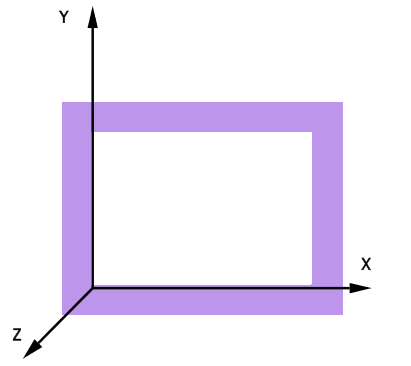
\includegraphics[width=3cm]
		{graphics/rhcoords}}
	\caption{\label{fig:rhcoords} Coordinate system assumed throughout module}
	\end{figure}
The default coordinate system assumed is right-handed: the positive x and y axes point right and up, and the negative z axis points forward. Positive rotation is counterclockwise about the axis of rotation.
\newline
Polygon Table consistency checks:
\begin{enumerate}
	\item Every vertex is listed as an endpoint of at least two edges
	\item Every surface is closed
	\item Each surface has at least one shared edge
\end{enumerate}
The order the vertices/edges are listed in a Geometric Polygon table do matter. Vertices written in clockwise order represent a surface pointing outwards. Whereas listing them counterclockwise represents an inwards pointing surface.

Meshes are a wireframe representation in which all vertices form a single set of continuous triangles, and all edges are a part of at least two triangles. Meshes can be generated by triangulation; but we covered just Delaunay Triangulation, defined above.
Meshes can also be progressive. Detail in meshes is unnecessary at farther distances, so vertices can be removed and added to create less detailed or more detailed meshes, respectively. Progress meshes do this dynamically based on viewer distance.

There are a few ways to represent polygons in a space, with boundary representations being only one method.
\begin{enumerate}
	\item Boundary Representation: Using vertices and drawing edges and surfaces from them
	\item Volumetric Models: Using simple shapes and various operations to create more complex shapes
	\item Implicit Models: Using implicit equations, such as that of a sphere, to generate shapes
	\item Parametric Models: Uses parametric equations to plot the multiple axes of a shape
\end{enumerate}
   \begin{figure}[!htb]
	\center{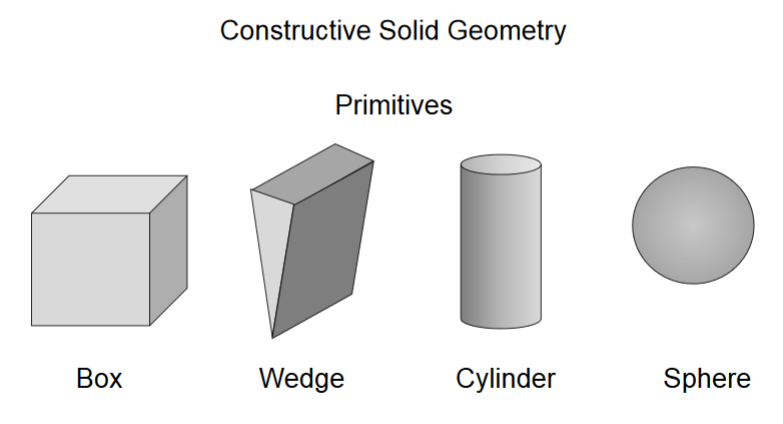
\includegraphics[width=10cm]
		{graphics/csg}}
	\caption{\label{fig:csg} Constructive Solid Geometry (CSG) Primitives}
\end{figure}
We covered a few volumetric models in the module.
\begin{enumerate}
	\item CSG: Uses primitve shapes and combines them uses set operations (union, difference, exclude, etc.) to generate new, more complex shapes.
	\item Voxels: 3D Pixels, unit cubes
	\item Octrees: Quad trees that divide in 3D space. Individual partitions are voxels
	\item Sweep: Using a 2D shape, moves that shape across a path, generating a volume in position the 2D shape occupies during its path
\end{enumerate}
One can also use implicit or parametric equations to generate shapes. Below is a list of equations that are common.
\begin{center}
	2D Circle:
	\begin{equation}
	\label{eqn:2dcirc}
	\left ( \frac{x}{r} \right )^2 + \left ( \frac{y}{r} \right )^2 = 1
	\end{equation}
	
	2D Circle - Parametric:
	\begin{equation}
	\label{eqn:2dcircpara}
	\begin{split}
	x = r\cos{\theta}  \\ y = r\sin{\theta} \\ -\pi \leq \theta \leq \pi
	\end{split}
	\end{equation}
	
	2D Ellipse - Parametric:
		\begin{equation}
	\label{eqn:2dellipsepara}
	\begin{split}
	x = r_x\cos{\theta}  \\ y = r_y\sin{\theta} \\ -\pi \leq \theta \leq \pi
	\end{split}
	\end{equation}
	
	3D Sphere:
	\begin{equation}
	\label{eqn:3dsphere}
	\left ( \frac{x}{r} \right )^2 + \left ( \frac{y}{r} \right )^2 + \left ( \frac{z}{r} \right )^2 = 1
	\end{equation}
	
	3D Ellipsoid:
	\begin{equation}
	\label{eqn:3dellipse}
	\left ( \frac{x}{r_x} \right )^2 + \left ( \frac{y}{r_y} \right )^2 + \left ( \frac{z}{r_z} \right )^2 = 1
	\end{equation}
	
	3D Sphere - Parametric:
	\begin{equation}
	\label{eqn:3dspherepara}
	\begin{split}
	x = r\cos{\phi}\cos{\theta}  \\ y = r\cos{\phi}\sin{\theta} \\ z = r\sin{\phi}\\ -\pi \leq \theta \leq \pi \\ -\pi/2 \leq \phi \leq \pi/2
	\end{split}
	\end{equation}
	
	3D Ellipsoid - Parametric:
	\begin{equation}
	\label{eqn:3dspherepara}
	\begin{split}
	x = r_x\cos{\phi}\cos{\theta}  \\ y = r_y\cos{\phi}\sin{\theta} \\ z = r_z\sin{\phi}\\ -\pi \leq \theta \leq \pi \\ -\pi/2 \leq \phi \leq \pi/2
	\end{split}
	\end{equation}
\end{center}

\subsection{Examples}
   \begin{figure}[!htb]
	\center{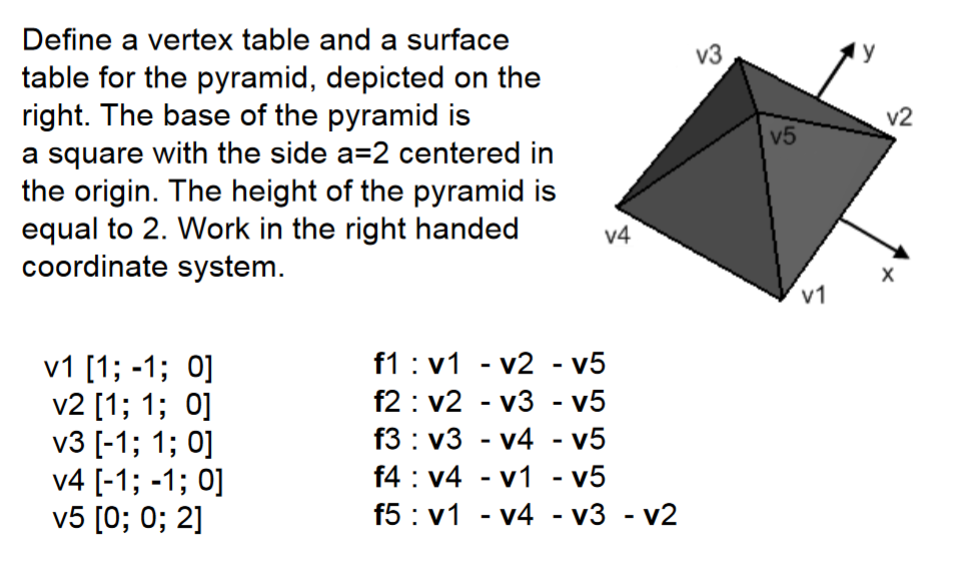
\includegraphics[width=15cm]
		{graphics/polygonTable}}
	\caption{\label{fig:pyramidPolygons} Example from Lecture}
	\end{figure}
Further Examples are taken from quizzes and assignments
\subsection{Further Sources}
	\href{https://www.tutorialspoint.com/computer_graphics/computer_graphics_surfaces.htm}{Surface Representations}
\newpage
\section{Transforms}
\newpage
\section{Lighting}
\newpage
\section{Projection}
\newpage
\section{Texture Mapping}
\newpage
\section{Past Exam Practice}